\setchapterstyle{kao}
\setchapterpreamble[u]{\margintoc}

\chapter{Hardware and Setup}

\section{The Microcontroller}

The first logical step for any embedded project is to select the proper hardware. The project's budget was relatively low, and previous experience with microcontroller programming was limited to 8-bit AVR \glspl{mcu}, which narrowed down the range of options to only a few possible controllers. Additionally, \glspl{mcu} which are already part of a development board like an Arduino were preferred because they do not need an external programming device.

The biggest challenge was to find an \gls{mcu} with sufficient PWM capabilities. Each simultaneously played tone requires an independent hardware timer with variable frequency and duty cycle, ideally 16 bit for better accuracy. Apart from the timers for tone generation, one more timer was needed to control the length of each tone. Because of the way the \gls{midi} protocol works, only one timer is needed for any amount of simultaneous notes. Since the human ear is much more sensitive to slightly wrong frequencies than slightly too short or too long notes, an 8 bit timer should be accurate enough. Table \ref{tab:mcu-selection} shows that the ATmega2560, the heart of the Arduino Mega, is best suited for this task because it has the most 16 bit timers.

\begin{margintable}[-1cm]
\centering

\caption{MCU Timer Comparison\label{tab:mcu-selection}}
\begin{tabular}{ccc}
    \multirow{2}*{\textbf{MCU}} & \multicolumn{2}{c}{\textbf{Timer}}\\\cmidrule{2-3}
           & 8-bit & 16-bit\\\midrule
    ATtiny85   & 2 & 0 \\
    ATmega328  & 2 & 1 \\
    ATmega32U4 & 1 & 2 \\
    ATmega2560 & 2 & 4 \\
\end{tabular}
\end{margintable}

\section{Programming Environment}

In order to have the maximum amount of flexibility for configuring the hardware, the programming language C\texttt{++} was chosen over the Arduino Language\sidenote{Especially because some Arduino libraries tend to break once the hardware it relies on has been configured manually.}. To avoid possible headaches while writing the code, the whole project was version controlled by git.

The toolchain used for compiling and uploading was the open source tool PlatformIO. It offers a simple interface to program a wide variety of \glspl{mcu} as well as a command line tool for more advanced tasks.

\newpage
\section{The Schematic}

Figure \ref{fig:fritzing} shows the complete schematic of the project, created with the open source circuit drawing tool \emph{fritzing}. Additionally, table \ref{tab:schematic-pins} shows all connections in tabular form.

\begin{figure}[h!]
    \centering
    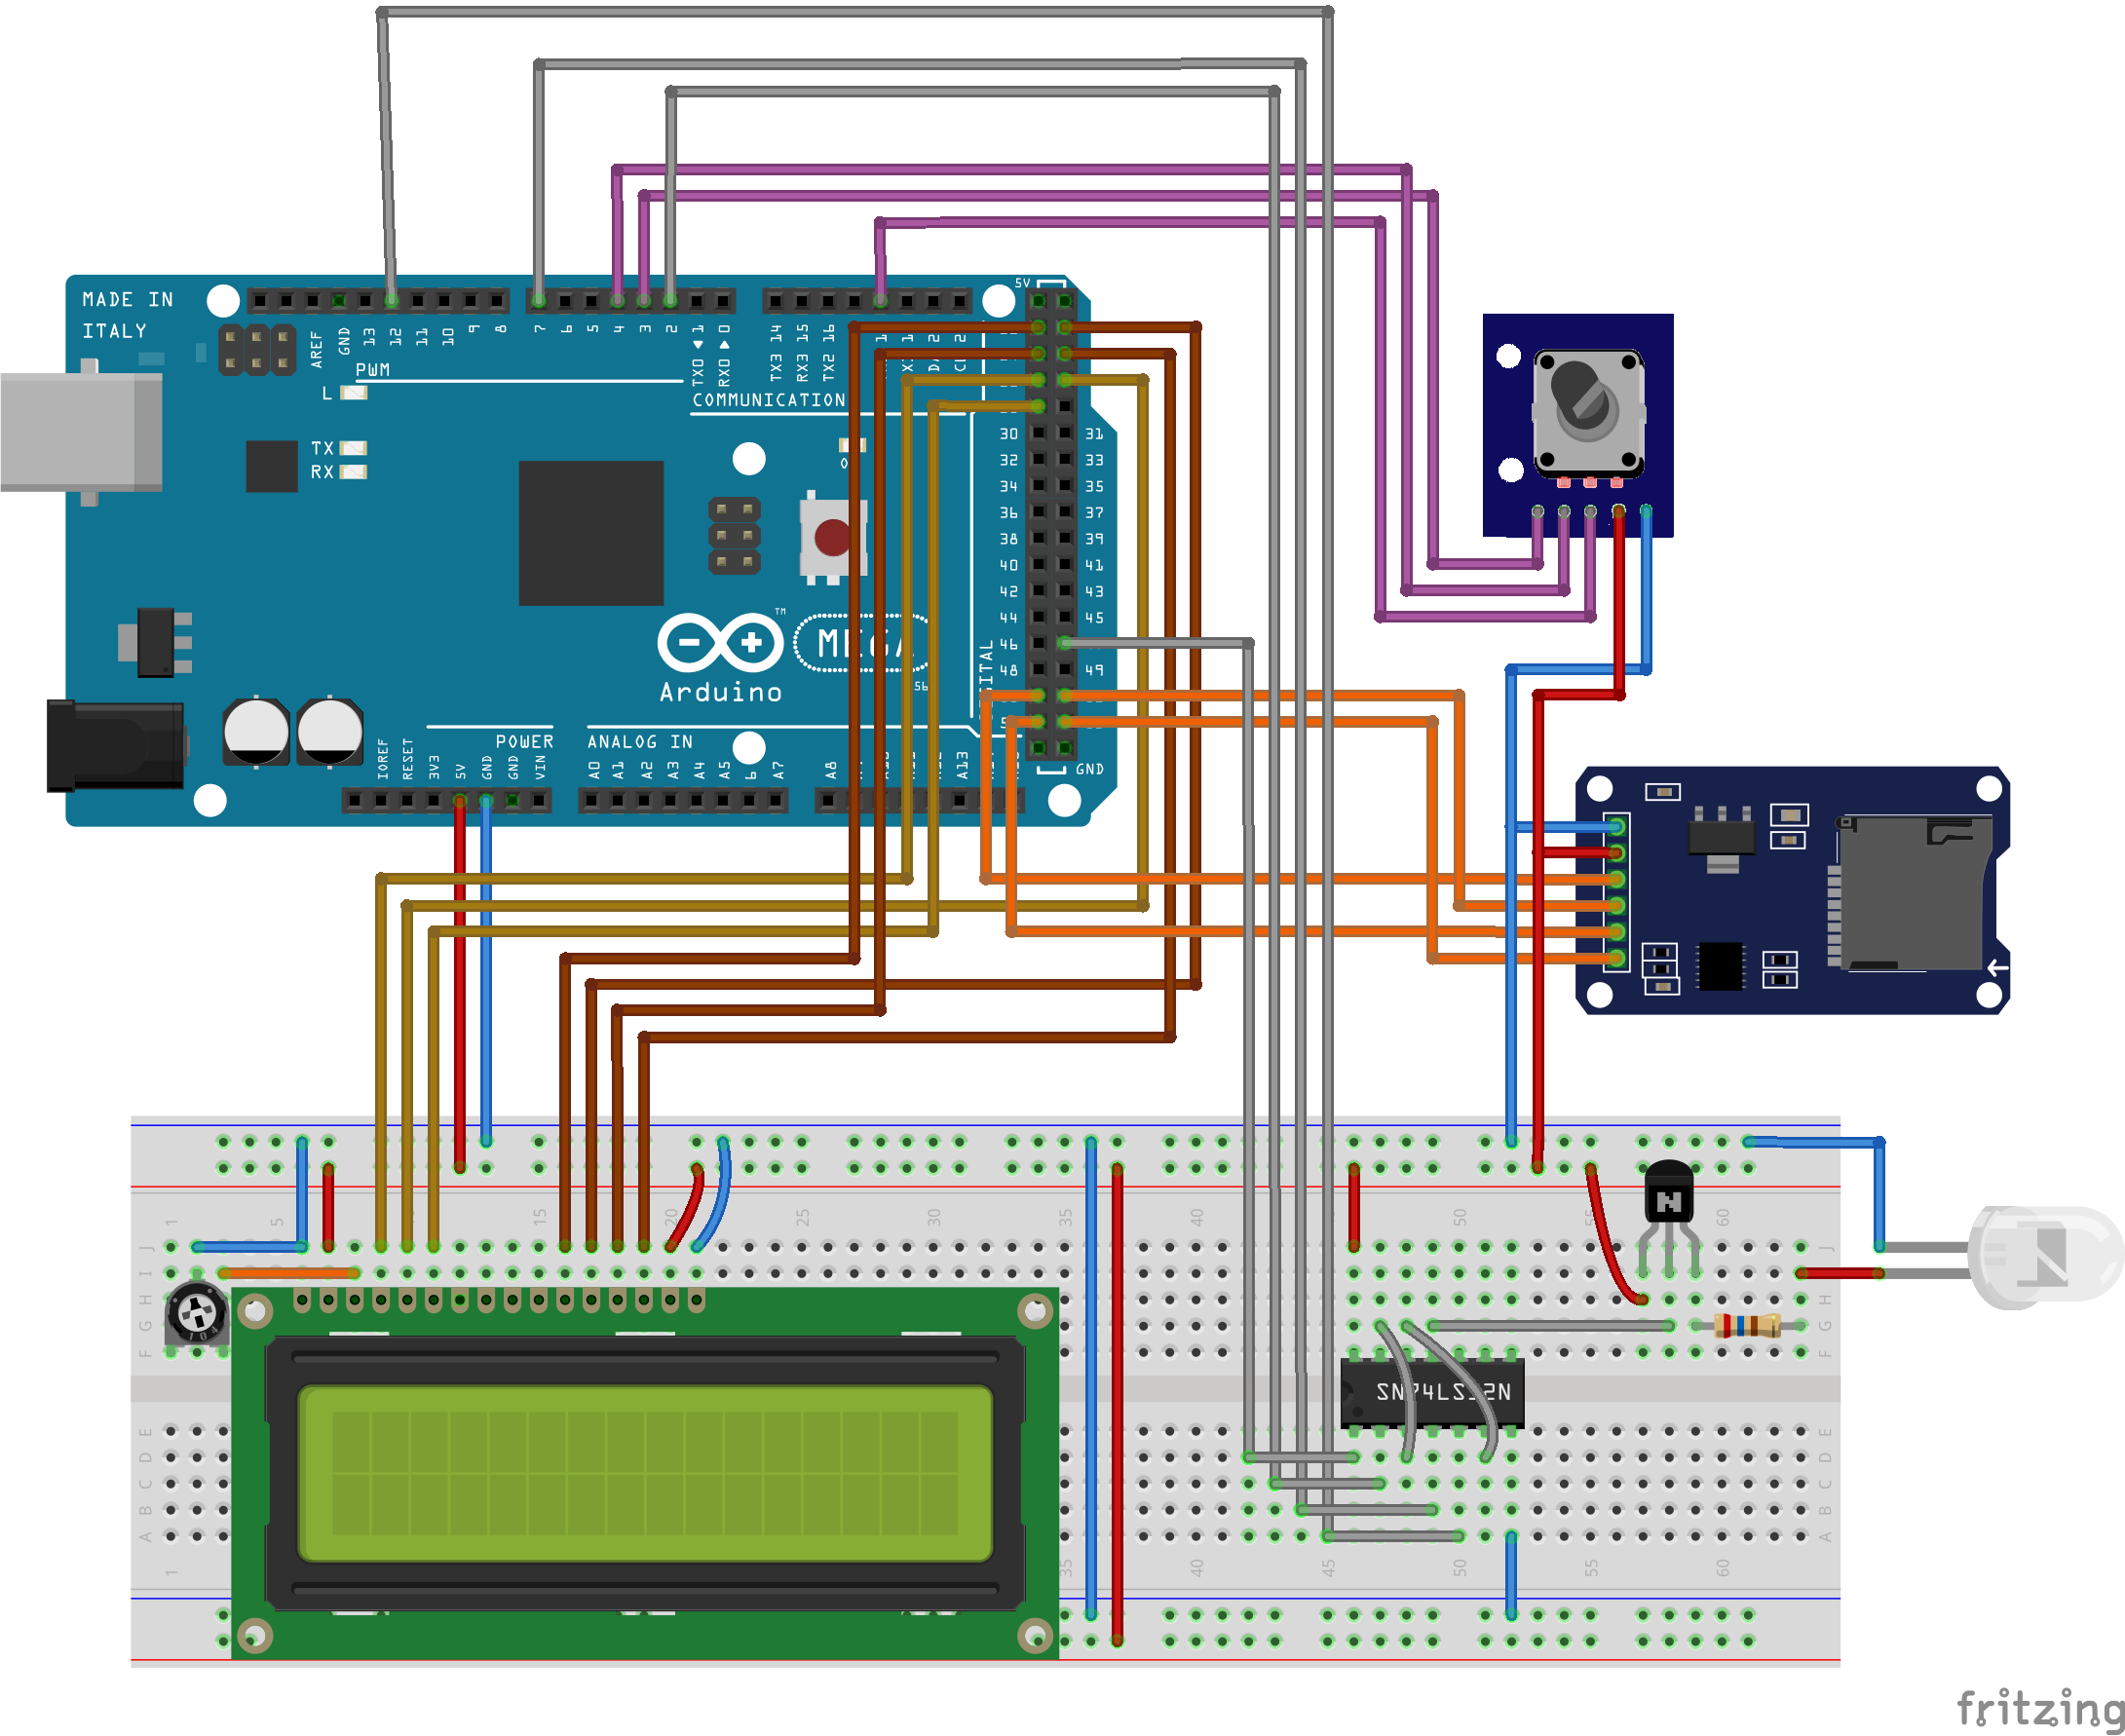
\includegraphics[width=0.95\textwidth]{felix/resources/fritzing.png}
    \caption{Complete Schematic}
    \label{fig:fritzing}
\end{figure}

\begin{margintable}[-14cm]
\centering
\label{tab:schematic-pins}
\caption{Connections}
\begin{tabular}{@{}crcl@{}}
\toprule
MCU & Arduino & \multicolumn{2}{c}{Device}           \\ \midrule
PB6     & 12          & \multirow{4}{*}{\rotatebox{90}{PWM}}         & C 1 \\
PE4     & 2           &                              & C 2 \\
PH4     & 7           &                              & C 3 \\
PL4     & 39          &                              & C 4 \\ \cmidrule{3-4}
PB0     & 53          & \multirow{4}{*}{\rotatebox{90}{SD card}}     & CS        \\
PB1     & 52          &                              & SCK       \\
PB2     & 51          &                              & MOSI      \\
PB3     & 50          &                              & MISO      \\ \cmidrule{3-4}
PA4     & 26          & \multirow{7}{*}{\rotatebox{90}{LCD}}        & RS        \\
PA5     & 27          &                              & RW        \\
PA6     & 28          &                              & E         \\
PA0     & 22          &                              & D4        \\
PA1     & 23          &                              & D5        \\
PA2     & 24          &                              & D6        \\
PA3     & 25          &                              & D7        \\ \cmidrule{3-4}
PE5     & 3           & \multirow{3}{*}{\rotatebox{90}{\parbox{13mm}{\centering Rotary\\Encoder}}} & CLK \\
PG5     & 4           &                              & DT        \\
PD3     & 18          &                              & SW        \\ \bottomrule
\end{tabular}
\end{margintable}

As shown, all devices were connected using a breadboard and jumper wires. Even though special care was taken that the jumper wires did not have a loose contact, they still caused connection issues and led to long searches for alleged software bugs. To stabilize the parts and keep them in position, they were screwed onto a wooden board. 
